\documentclass[]{book}

%These tell TeX which packages to use.
\usepackage{array,epsfig}
\usepackage{amsmath}
\usepackage{amsfonts}
\usepackage{amssymb}
\usepackage{amsxtra}
\usepackage{amsthm}
\usepackage{mathrsfs}
\usepackage{color}
\usepackage{pgfplots}

%Here I define some theorem styles and shortcut commands for symbols I use often
\theoremstyle{definition}
\newtheorem{defn}{Definition}
\newtheorem{thm}{Theorem}
\newtheorem{cor}{Corollary}
\newtheorem*{rmk}{Remark}
\newtheorem{lem}{Lemma}
\newtheorem*{joke}{Joke}
\newtheorem{ex}{Example}
\newtheorem*{soln}{Solution}
\newtheorem{prop}{Proposition}

\newcommand{\lra}{\longrightarrow}
\newcommand{\ra}{\rightarrow}
\newcommand{\surj}{\twoheadrightarrow}
\newcommand{\graph}{\mathrm{graph}}
\newcommand{\bb}[1]{\mathbb{#1}}
\newcommand{\Z}{\bb{Z}}
\newcommand{\Q}{\bb{Q}}
\newcommand{\R}{\bb{R}}
\newcommand{\C}{\bb{C}}
\newcommand{\N}{\bb{N}}
\newcommand{\M}{\mathbf{M}}
\newcommand{\m}{\mathbf{m}}
\newcommand{\MM}{\mathscr{M}}
\newcommand{\HH}{\mathscr{H}}
\newcommand{\Om}{\Omega}
\newcommand{\Ho}{\in\HH(\Om)}
\newcommand{\bd}{\partial}
\newcommand{\del}{\partial}
\newcommand{\bardel}{\overline\partial}
\newcommand{\textdf}[1]{\textbf{\textsf{#1}}\index{#1}}
\newcommand{\img}{\mathrm{img}}
\newcommand{\ip}[2]{\left\langle{#1},{#2}\right\rangle}
\newcommand{\inter}[1]{\mathrm{int}{#1}}
\newcommand{\exter}[1]{\mathrm{ext}{#1}}
\newcommand{\cl}[1]{\mathrm{cl}{#1}}
\newcommand{\ds}{\displaystyle}
\newcommand{\vol}{\mathrm{vol}}
\newcommand{\cnt}{\mathrm{ct}}
\newcommand{\osc}{\mathrm{osc}}
\newcommand{\LL}{\mathbf{L}}
\newcommand{\UU}{\mathbf{U}}
\newcommand{\support}{\mathrm{support}}
\newcommand{\AND}{\;\wedge\;}
\newcommand{\OR}{\;\vee\;}
\newcommand{\Oset}{\varnothing}
\newcommand{\st}{\ni}
\newcommand{\wh}{\widehat}

%Pagination stuff.
\setlength{\topmargin}{-.3 in}
\setlength{\oddsidemargin}{0in}
\setlength{\evensidemargin}{0in}
\setlength{\textheight}{9.in}
\setlength{\textwidth}{6.5in}
\pagestyle{empty}



\begin{document}

\subsection*{Exo 1}
Rappel de cours:
\begin{itemize}
\item Une fonction d\'erivable est continue, par contre le r\'eciproque n'est pas vraie
\item Une fonction est d\'erivable sur un intervalle si elle est d\'erivable en tout point de cette intervalle
\item Une fonction est d\'erivable en un point $a$ si $\exists l, \lim_{x \to a}\frac{f(x)-f(a)}{x-a} = l$ ou $\exists l, \lim_{h \to 0}\frac{f(a+h)-f(a)}{h}$
\item une fonction est d\'erivable sur un intervalle donné si elle est un assemblage de fonctions connues et dérivables sur cette intervalle.
\end{itemize}

La fonction $f(x) = |x-\pi| sin(x)$ est \'egale \`a
$$f(x) = 
\left\{ 
\begin{array}{l l}
 (x-\pi) sin(x) & x \ge \pi \\
 (\pi-x) sin(x) & x < \pi \\
\end{array}
\right. 
$$

Les deux parties sont un assemblage fonctions d\'erivables sur leur intervalle. Il reste \`a d\'emontrer si la fonction est d\'erivable en $\pi$.
$$\exists l, \lim_{x \to \pi}\frac{f(x)-f(\pi)}{x-\pi} = l$$
$$ 
\left\{ 
\begin{array}{l}
 \lim_{x \to \pi^{+}}\frac{(x-\pi) sin(x) - (\pi-\pi) sin(\pi)}{x-\pi} \\
 \lim_{x \to \pi^{-}}\frac{(\pi-x) sin(x) - (\pi-\pi) sin(\pi)}{x-\pi} \\
\end{array}
\right. 
$$

$$ 
\left\{ 
\begin{array}{l}
 \lim_{x \to \pi^{+}}\frac{(x-\pi) sin(x)}{x-\pi} \\
 \lim_{x \to \pi^{-}}\frac{-(x-\pi) sin(x)}{x-\pi} \\
\end{array}
\right. 
$$

$$ 
\left\{ 
\begin{array}{l}
 \lim_{x \to \pi^{+}} sin(x) \\
 \lim_{x \to \pi^{-}} -sin(x) \\
\end{array}
\right. 
$$

La fonction sinus est impaire, $sin(-x) = -sin(x)$. Donc

$$ 
\left\{ 
\begin{array}{l}
 \lim_{x \to \pi^{+}} sin(x) \\
 \lim_{x \to \pi^{-}} sin(-x) \\
\end{array}
\right. 
$$

on a $\lim_{x \to \pi^{-}} sin(-x) = \lim_{x \to \pi^{+}} sin(x)$. La valeur $l$ existe donc la fonction $f$ est d\'erivable.\\

La proposition est Vraie.

\subsection*{Exo 2}

Soit $f(x) = e^{x}$. on a $\forall x, f'(x) = e^{x}$
$$\lim_{h \to 0}\frac{f(x_0+3h)-f(x_0+h)}{h}$$
$$\lim_{h \to 0}\frac{e^{(x_0+3h)} - e^{(x_0+h)}}{h}$$
$$\lim_{h \to 0}\frac{e^{x_0}.e^{3h} - e^{x_0}.e^{h}}{h}$$
$$\lim_{h \to 0}\frac{e^{x_0}(e^{3h}-e^{h})}{h}$$
$$e^{x_0}\lim_{h \to 0}\frac{(e^{3h}-e^{h})}{h}$$

Si $\lim_{h \to 0}\frac{f(x_0+3h)-f(x_0+h)}{h} = 2f'(x_0)$ alors on a $\lim_{h \to 0}\frac{(e^{3h}-e^{h})}{h} = e^{x_0}$. Ce qui est faux.\\

La proposition est Fausse.

\subsection*{Exo 3}
Comme $f$ est d\'erivable, on peut \'ecrire son d\'eveloppement limit\'e d'ordre 1 en $0$; $f(x) - f(0) = f'(0)(x - 0) + (x - 0)\epsilon(x - 0)$

On a $f(0) = e^{sin(2.0)} = 1$, $f'(x) = 2cos(2x)e^{sin(2x)}$, donc $f'(0) = 2$. Donc $f(x) = 1 + 2x + x\epsilon(x) \neq 1 + 3x + x\epsilon(x) $.\\

La proposition est Fausse.


\subsection*{Exo 4}
Soit $f(x) = (x-1)^3$, le fonction est d\'erivable $f'(x)=3(x-1)^2$ et $f'(1) = 0$. Le point $1$ n'est pas un extremum de la fonction sur l'intervalle $[-2,3]$. En effet, $f(-2) = -27 < f(1) = 0$ donc $1$ n'est pas un minimum local et $f(3) = 8 > f(1) = 0$ donc $1$ n'est pas un maximum local.\\

La proposition est Fausse.\\

\begin{tikzpicture}
	\begin{axis}[
        axis lines = middle,
		xlabel=$x$,
		ylabel={$f(x) = (x-1)^3$},
		grid=major,
	]
	% use TeX as calculator:
	\addplot [
   domain=-2:3,
   samples=100,
   color=blue]
   {(x-1)^3};
	\end{axis}
\end{tikzpicture}



\subsection*{Exo 5}
Soit $f(x) = |x|$, la fonction est d\'efinie et continue en $0$ mais pas d\'erivable en $0$.
En effet, si $f(x)$ est d\'erivable en $a$ alors, $\exists l, \lim_{x \to a}\frac{f(x)-f(a)}{x-a} = l$

$$ 
\left\{ 
\begin{array}{l}
 \lim_{x \to 0^{+}} \frac{x - 0}{x-0} = 1 \\
 \lim_{x \to 0^{-}} \frac{-x - 0}{x-0} = -1 \\
\end{array}
\right. 
$$

La proposition est Fausse.

\subsection*{Exo 6}
La fonction $tan^3(x)$ est d\'erivable sur $]-\frac{\pi}{2},\frac{\pi}{2}[$ car c'est un asssemblage de fonctions d\'erivable sur cette intervalle.

$$(tan^3(x))' = 3(tan(x))'tan^2(x)=3(1+tan^2(x))tan^2(x) = 3(tan^2(x)+tan^4(x))$$

La proposition est Fausse.


\subsection*{Exo 7}
Calculons la d\'eriv'ee de $h(x) = \frac{x}{\sqrt{1+x^2}}$.
$$
\begin{array}{l l}
 f(x) = x & f'(x) = 1 \\
 g(x) = \sqrt{1+x^2} & g'(x) = \frac{x}{\sqrt{1+x^2}} \\
\end{array}
$$

$h'(x) = \frac{1.\sqrt{1+x^2} - x.\frac{x}{\sqrt{1+x^2}}}{1+x^2} = \frac{\frac{1}{\sqrt{1+x^2}}}{1+x^2} = \frac{1}{(1+x^2)\sqrt{1+x^2}}$.

La fonction $h$ n'a pas de maximum ou minimum si sa d\'eriv\'ee ne peux pas \^etre nulle; $\forall x \in \R, h'(x) \neq 0$.
$$ \frac{1}{(1+x^2)\sqrt{1+x^2}} = 0 $$
$$ 1 = 0 $$


OU
La fonction $h(x) = \frac{x}{\sqrt{1+x^2}}$ est strictement croissante. Donc le maximum de $h(x)$, si il existe, est la limite quand $X \to +\infty$ et le minimum de $h(x)$, si il existe, est la limite quand $X \to -\infty$.
Remarquons que, $\forall x \in \R, x^2 < 1 + x^2$ donc $\forall x \in \R, |x| < \sqrt{1 + x^2}$ et $\forall x \in \R, \frac{|x|}{\sqrt{1 + x^2}} < 1$.\\
 
Lorsque $x \to +\infty$, $h(x)$ s'approche arbitrairement pr\`es de la valeur $1$ mais sans jamais atteindre cette valeur. Donc, $f(x)$ n'admet pas de maximum.\\

Lorsque $x \to -\infty$, $h(x)$ s'approche arbitrairement pr\`es de la valeur $-1$ mais sans jamais atteindre cette valeur. Donc, $f(x)$ n'admet pas de minimum.\\


La proposition est Vraie.



\subsection*{Exo 8}
On a $\lim_{x \to +\infty} x + 2sin(x) = +\infty$ et $\lim_{x \to -\infty} x + 2sin(x) = -\infty$. Donc la fonction n'a pas de minima ou de maxima sur $\R$.\\

La proposition est Fausse.\\

Note: la d\'eriv\'ee de $f$ s'annule une infinit\'e de fois. Donc, $f'(x)=0$ n'implique pas qu'il existe un maximum ou un minimum.


\subsection*{Exo 9}
Preuve par l'absurde. \\

Admettons que la fonction $f$ ne soit pas born\'ee sur l'intervalle $[0,1]$, donc elle n'admet pas de valeur maximale (resp. minimale) sur l'intervalle $[0,1]$; $\exists c \in [0,1], f(c) = +\infty\, (resp.\, -\infty)\,\,\,[1]$.\\

La fonction $f$ est continue sur l'intervalle $[0,1]$, donc $\forall x_0 \in [0,1], \forall \epsilon >0, \exists \eta > 0\; tel\; que\; (\forall x \in [0,1] \cap ]x_0-\eta, x_0+\eta[, |f(x)-f(x_0)| < \epsilon)\,\,\,[2]$. \\ 

Au point $c$, la proposition $[2]$ est fausse, la fonction $f$ admet une valeur maximale $M$ (resp. minimale $m$) sur l'intervalle $[0,1]$. Donc la fonction $f$ est born\'ee.\\


On peut \'egalement utiliser le th\'eor\`eme de Bolzano-Weierstrass.\\

La proposition est Vraie.

\subsection*{Exo 10}
Preuve par l'absurde. \\

Admettons que la fonction $f$ n'a pas de valeur maximale sur l'intervalle $[0,1]$, donc $\exists c \in [0,1], f(c) = +\infty\,\,\,[1]$.\\

La fonction $f$ est continue sur l'intervalle $[0,1]$, donc $\forall x_0 \in [0,1], \forall \epsilon >0, \exists \eta > 0\; tel\; que\; (\forall x \in [0,1] \cap ]x_0-\eta, x_0+\eta[, |f(x)-f(x_0)| < \epsilon)\,\,\,[2]$. \\ 

Au point $c$, la proposition $[2]$ est fausse, la fonction $f$ admet une valeur maximale sur l'intervalle $[0,1]$.\\


On peut \'egalement utiliser le th\'eor\`eme de Bolzano-Weierstrass.\\

La proposition est Vraie.


\subsection*{Exo 11}
Preuve par l'absurde. \\

Soit une fonction $f$ p\'eriodique de p\'eriode $p$ et continue. \\

Admettons que la fonction $f$ n'a pas de valeur maximale sur l'intervalle $[0,p]$, donc $\exists c \in [0,p], f(c) = +\infty\,\,\,[1]$.\\

La fonction $f$ est continue sur $\R$ donc \'egalement sur l'intervalle $[0,p]$, donc $\forall x_0 \in [0,p], \forall \epsilon >0, \exists \eta > 0\; tel\; que\; (\forall x \in [0,p] \cap ]x_0-\eta, x_0+\eta[, |f(x)-f(x_0)| < \epsilon)\,\,\,[2]$. \\ 

Au point $c$, la proposition $[2]$ est fausse, la fonction $f$ admet une valeur maximale sur l'intervalle $[0,p]$. Comme la fonction est p\'eriodique, on a $\forall x \in \R, f(x) = f(x\%p)$, et $x\%p \in [0,p]$, donc la valeur maximale sur l'intervalle $[0,p]$ est \'egalement la valeur maximale de la fonction $f$ sur $\R$. \\


On peut \'egalement utiliser le th\'eor\`eme de Bolzano-Weierstrass.\\

La proposition est Vraie.

\subsection*{Exo 12}
Montrons:
$$\forall x,y \in [-1,1],|x^{2013} - y^{2013}| \le 2013|x-y|$$
$|x-y| \ge 0$, donc
$$\forall x,y \in [-1,1],\frac{|x^{2013} - y^{2013}|}{|x-y|} \le 2013$$
$$\forall x,y \in [-1,1],\Big| \frac{x^{2013} - y^{2013}}{x-y} \Big| \le 2013$$
$$\forall x,y \in [-1,1], |\sum_{k=0}^{2012}x^k.y^{2012-k}| \le 2013$$

On a $x,y \in [-1,1]$, donc $x^m,y^m \in [-1,1]$ et $x^m.y^m \in [-1,1]$. Donc $\sum_{k=0}^{2012}x^k.y^{2012-k} \in [-2013,2013]$ et $|\sum_{k=0}^{2012}x^k.y^{2012-k}| \le 2013$.
\\

La proposition est Vraie.

\subsection*{Exo 13}


\subsection*{Exo 14}
Prenons la valeur $x = -\frac{\pi}{2}$, on a $cos(-\frac{\pi}{2})-1 = -1 \nleq -\frac{\pi}{2}$.\\


La proposition est Fausse.


\subsection*{Exo 15}
La function $ln$ est strictement croissante, donc $\frac{ln\,a}{ln\,b} < 1$ car $a<b$. Pour que l'\'egalit\'e soit vraie, il faut que $\frac{a-b}{c.ln(c)} < 0$ car $e^{\frac{a-b}{c.ln(c)}} < 1$.\\
On a $a-b < 0$ car $a<b$, donc il faut que $c.ln(c)$ soit positif. Ceci est vrai lorsque $c > 1$.\\


La proposition est Vraie.


\subsection*{Exo 16}
Rappel de cours:\\
La fonction $f$ est de classe $\C^1$ sur l'intervalle $I$ si la fonction est d\'erivable sur $I$ et que sa d\'eriv\'e est continue sur $I$.

$$f: \R \to \R,
\left\{ 
\begin{array}{l l}
 x^2sin(\frac{1}{x}) & x \neq 0\\
 0 & x = 0\\
\end{array}
\right. 
$$

La fonction $f$ est d\'erivable sur $\R$ car c'est un assemblage de fonctions d\'erivables. Calculons la d\'eriv\'ee de $f$.
$$
\begin{array}{l l}
 h(x) = x^2 & h'(x)= 2x\\
 g(x) = sin(\frac{1}{x}) & g'(x)= -\frac{1}{x^2}cos(\frac{1}{x})\\
\end{array}
$$

Donc,
$$f': \R \to \R,
\left\{ 
\begin{array}{l l}
 (x^2)(-\frac{1}{x^2}cos(\frac{1}{x})) + 2x.sin(\frac{1}{x}) = 2x.sin(\frac{1}{x}) - cos(\frac{1}{x})& x \neq 0\\
 0 & x = 0\\
\end{array}
\right. 
$$

Il faut maintenant v\'erifier que la d\'eriv\'ee $f'(x)$ est continue sur $\R$. Pour $x \neq 0$, la fonction est continue car c'est un assemblage de fonctions continues, pour $x=0$, la fonction est \'egalement continue. Il reste \`a v\'erifier que la fonction est continue en $0$; $\lim_{x \to 0} 2x.sin(\frac{1}{x}) - cos(\frac{1}{x}) = 0$?\\

La fonction $cos(\frac{1}{x})$ n'a pas de limite en $0$.\\

La proposition est Fausse.


\end{document}

